\documentclass[]{article}
\usepackage{lmodern}
\usepackage{amssymb,amsmath}
\usepackage{ifxetex,ifluatex}
\usepackage{fixltx2e} % provides \textsubscript
\ifnum 0\ifxetex 1\fi\ifluatex 1\fi=0 % if pdftex
  \usepackage[T1]{fontenc}
  \usepackage[utf8]{inputenc}
\else % if luatex or xelatex
  \ifxetex
    \usepackage{mathspec}
  \else
    \usepackage{fontspec}
  \fi
  \defaultfontfeatures{Ligatures=TeX,Scale=MatchLowercase}
\fi
% use upquote if available, for straight quotes in verbatim environments
\IfFileExists{upquote.sty}{\usepackage{upquote}}{}
% use microtype if available
\IfFileExists{microtype.sty}{%
\usepackage{microtype}
\UseMicrotypeSet[protrusion]{basicmath} % disable protrusion for tt fonts
}{}
\usepackage[margin=1in]{geometry}
\usepackage{hyperref}
\hypersetup{unicode=true,
            pdftitle={assignment6},
            pdfauthor={guanxuyi},
            pdfborder={0 0 0},
            breaklinks=true}
\urlstyle{same}  % don't use monospace font for urls
\usepackage{graphicx,grffile}
\makeatletter
\def\maxwidth{\ifdim\Gin@nat@width>\linewidth\linewidth\else\Gin@nat@width\fi}
\def\maxheight{\ifdim\Gin@nat@height>\textheight\textheight\else\Gin@nat@height\fi}
\makeatother
% Scale images if necessary, so that they will not overflow the page
% margins by default, and it is still possible to overwrite the defaults
% using explicit options in \includegraphics[width, height, ...]{}
\setkeys{Gin}{width=\maxwidth,height=\maxheight,keepaspectratio}
\IfFileExists{parskip.sty}{%
\usepackage{parskip}
}{% else
\setlength{\parindent}{0pt}
\setlength{\parskip}{6pt plus 2pt minus 1pt}
}
\setlength{\emergencystretch}{3em}  % prevent overfull lines
\providecommand{\tightlist}{%
  \setlength{\itemsep}{0pt}\setlength{\parskip}{0pt}}
\setcounter{secnumdepth}{0}
% Redefines (sub)paragraphs to behave more like sections
\ifx\paragraph\undefined\else
\let\oldparagraph\paragraph
\renewcommand{\paragraph}[1]{\oldparagraph{#1}\mbox{}}
\fi
\ifx\subparagraph\undefined\else
\let\oldsubparagraph\subparagraph
\renewcommand{\subparagraph}[1]{\oldsubparagraph{#1}\mbox{}}
\fi

%%% Use protect on footnotes to avoid problems with footnotes in titles
\let\rmarkdownfootnote\footnote%
\def\footnote{\protect\rmarkdownfootnote}

%%% Change title format to be more compact
\usepackage{titling}

% Create subtitle command for use in maketitle
\newcommand{\subtitle}[1]{
  \posttitle{
    \begin{center}\large#1\end{center}
    }
}

\setlength{\droptitle}{-2em}
  \title{assignment6}
  \pretitle{\vspace{\droptitle}\centering\huge}
  \posttitle{\par}
  \author{guanxuyi}
  \preauthor{\centering\large\emph}
  \postauthor{\par}
  \predate{\centering\large\emph}
  \postdate{\par}
  \date{March 30, 2018}


\begin{document}
\maketitle

\section{Bude \ldots{}}\label{bude}

is a small seaside resort town in north Cornwall, England, UK,\\
in the civil parish of Bude-Stratton and at the mouth of the River Neet
(also known locally as the River Strat). It is sometimes formerly known
as Bude Haven.{[}4{]} It lies southwest of Stratton, south of Flexbury
and Poughill, and north of Widemouth Bay and is located along the A3073
road off the A39. Bude is twinned with Ergué-Gabéric in Brittany,
France.{[}5{]} Bude's coast faces Bude Bay in the Celtic Sea, part of
the Atlantic Ocean. The population of the civil parish can be found
under Bude-Stratton.

\subsection{Watermap for Bude}\label{watermap-for-bude}

\includegraphics[width=400pt,height=350pt]{watermap.png}

\subsection{Roadmap image}\label{roadmap-image}

\includegraphics[width=400pt,height=350pt]{roadmap.png}

\section{There's a lot to love about
Bude!}\label{theres-a-lot-to-love-about-bude}

With a laidback allure all of its own, and so much to see and do, we
have something for everyone. From romantic whiskaways to fun-fuelled
family holidays, it's all here, where Cornwall begins and everyday cares
melt away. Bude has been named as the Best UK Coastal Resort for three
consecutive years, winning a section of Gold, Silver and Bronze awards
in the British Travel Awards. Below are some of the best locations for a
vacation getway.

\subsection{\texorpdfstring{\textbf{The Bude
Beaches}}{The Bude Beaches}}\label{the-bude-beaches}

\includegraphics[width=400pt,height=350pt]{BudeBeaches.jpg}

\subsection{\texorpdfstring{\textbf{The Summerleaze
Beach}}{The Summerleaze Beach}}\label{the-summerleaze-beach}

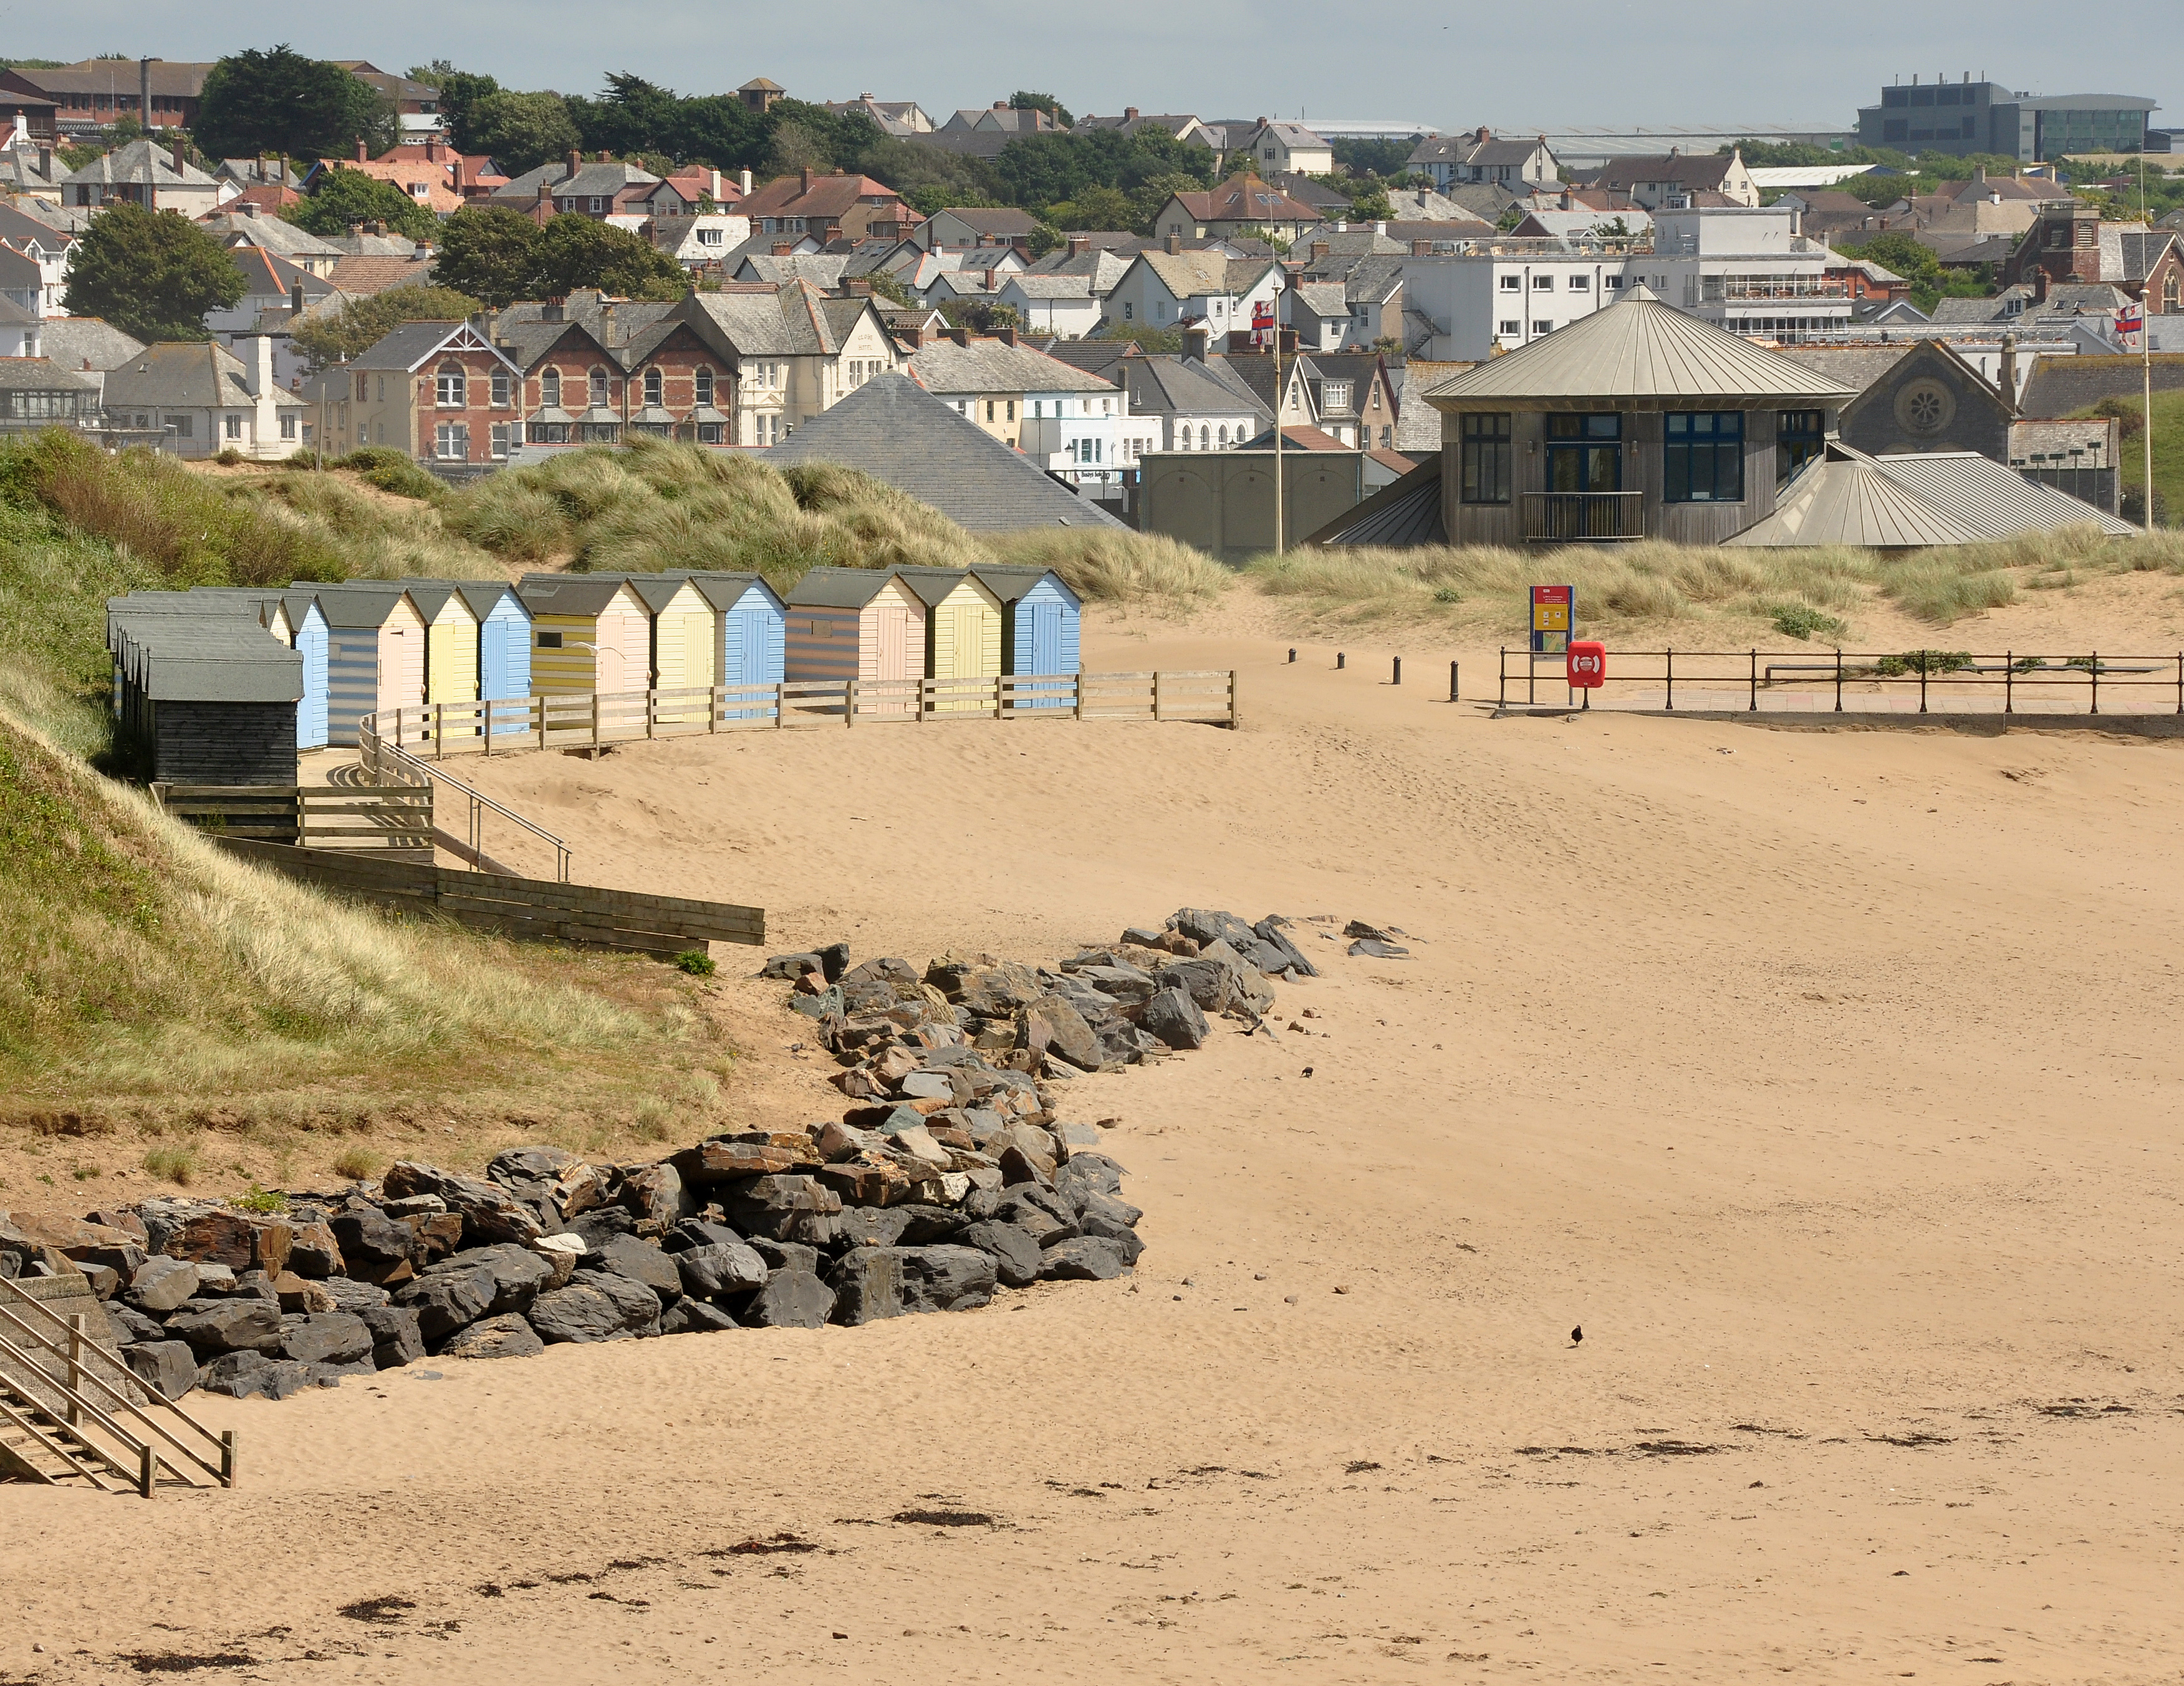
\includegraphics[width=400pt,height=350pt]{SummerleazeBeach.jpg}

\subsection{\texorpdfstring{\textbf{The Crooklets
Beach}}{The Crooklets Beach}}\label{the-crooklets-beach}

\includegraphics[width=400pt,height=350pt]{CrookletsBeach.jpg}

\section{Cricket by the Sea}\label{cricket-by-the-sea}

\subsection{\texorpdfstring{\textbf{The Bude North Cornwall Cricket
Club}}{The Bude North Cornwall Cricket Club}}\label{the-bude-north-cornwall-cricket-club}

\includegraphics[width=400pt,height=350pt]{BudeNorthCornwallCricketClub.jpg}

\subsection{\texorpdfstring{\textbf{The Barrel at
Bude}}{The Barrel at Bude}}\label{the-barrel-at-bude}

\includegraphics[width=400pt,height=350pt]{TheBarrelatBude.jpg}


\end{document}
